\documentclass[11pt, twoside]{article}

\usepackage{subcaption}
\usepackage{wrapfig}
\usepackage[utf8]{inputenc}
\usepackage[english]{babel}
\usepackage{mathptmx}
\usepackage{graphicx}
\usepackage{fancyhdr}
\usepackage{hyperref}
\usepackage{url}
\usepackage{icomma}
\usepackage{svg}
\graphicspath{{images/}}
\usepackage{footmisc}
\usepackage{listings}
\usepackage{titlesec}
\usepackage{afterpage}
\usepackage[top=2cm,tmargin=2cm,textheight=18cm,footnotesep=1.2cm,bottom=6cm]{geometry}
\usepackage{parskip}
\usepackage{lipsum}
\usepackage{tabularray}
\usepackage{amsmath}
\usepackage{tabu}
%\usepackage{siunitx}
\counterwithin{figure}{section}
\counterwithin{table}{section}
\numberwithin{equation}{section}
\usepackage{setspace}
\usepackage{listings}
\usepackage[labelfont=bf, skip=5pt, font=small]{caption}
\hypersetup{colorlinks=true, linkcolor=blue,filecolor=magenta, urlcolor=cyan, citecolor=blue}
\usepackage[style=apa, sorting=nyt]{biblatex}
\addbibresource{References.bib}
\usepackage[version=4]{mhchem}
\usepackage{pythontex}
\usepackage{enumitem}
\usepackage[dvipsnames, svgnames, usenames]{xcolor}
\usepackage{pdfpages}
\usepackage{cleveref}
\usepackage[T1]{fontenc}
\usepackage{tgpagella}

% For the DAG
\usepackage{tikz}
\usetikzlibrary{arrows.meta, positioning}

\lstset{language=Python, 
        basicstyle=\ttfamily\footnotesize, 
        keywordstyle=\color{blue}, 
        commentstyle=\color{green}, 
        breaklines=true,
        stringstyle=\color{red}}

\DeclareCaptionFormat{custom}
{\textbf{#1 #2}\textit{\small #3}}
\captionsetup{format=custom}

\newcommand{\lightgray}[1]{\colorbox{lightgray!40}{\texttt{\detokenize{#1}}}}

% Setlength
\setcounter{tocdepth}{4}
\setcounter{secnumdepth}{4}
\setlength{\parskip}{1em}
\setlength{\parindent}{0em}
\setstretch{0.1}
\setlist{itemsep=0\baselineskip}
\setlength{\skip\footins}{0.5cm}
\setlength{\headheight}{75pt}
\setlength{\belowdisplayskip}{0pt} 
\setlength{\belowdisplayshortskip}{0pt}
\setlength{\abovedisplayskip}{0pt} 
\setlength{\abovedisplayshortskip}{0pt}
\addtolength\abovedisplayskip{-0.5\baselineskip}
\addtolength\belowdisplayskip{-0.5\baselineskip}
\renewcommand{\baselinestretch}{1}\normalsize
%\sisetup{inter-unit-product =$\cdot$}

\newcommand\blankpage{%
    \null
    \thispagestyle{empty}%
    \addtocounter{page}{-1}%
    \newpage}

\crefname{figure}{Fig.}{Figs.}       % Enkelvoud en meervoud voor figuren
\Crefname{figure}{Fig.}{Figs.}       % Hoofdlettervariant
\crefname{table}{Tab.}{Tabs.}        % Enkelvoud en meervoud voor tabellen
\Crefname{table}{Tab.}{Tabs.}        % Hoofdlettervariant
\crefname{equation}{Eq.}{Eqs.}       % Enkelvoud en meervoud voor vergelijkingen
\Crefname{equation}{Eq.}{Eqs.}       % Hoofdlettervariant
\newcommand{\fullref}[1]{\hyperref[#1]{\Cref{#1}}}

\begin{document}

% Eerste pagina zonder fancyhdr en plain maken (normaal)
\thispagestyle{empty}  % Verberg header/footer op de eerste pagina
\pagestyle{fancy}      % Zet fancy header/footer voor de rest van het document

% Verhoog de baselinedichtheid
\renewcommand{\baselinestretch}{1}\normalsize

% Header en footer instellingen
\fancyhf{}  % Leeg de standaard header/footer
\renewcommand{\footrulewidth}{1.1pt}  % Voeg een voetregel toe
\renewcommand{\headrulewidth}{0pt}    % Geen regel in de header
\fancyhead[L]{
\includegraphics[width=0.3\textwidth]{HAN-merkteken-descriptor.png}}  % Linksboven
\fancyfoot[LE]{\thepage}  % Links onder pagina nummer (even pagina's)
\fancyfoot[RO]{\thepage}  % Rechts onder pagina nummer (oneven pagina's)
\fancyfoot[LO]{\leftmark}   % Voeg hoofdstuktitel toe in de voettekst
\fancyfoot[RE]{\leftmark}   % Voeg hoofdstuktitel toe in de voettekst

% Begin van het document
\begin{titlepage}
    \centering
    
\includegraphics[width=0.7\textwidth]{HAN-merkteken-descriptor.png}
    \vspace{1cm} % Voeg ruimte toe
    \hrule
    \vspace{0.5cm}
    {\Huge \bfseries Portfolio Assignment 2 - Ethics \par}
    \vspace{0.5cm}
    \hrule
    \vspace{0.5cm}
    {\LARGE Marcello Wienhoven \par}
    \vspace{0.5cm}
    {\LARGE \today \par}
    \vspace{0.5cm}
    \hrule
    
\end{titlepage}

\pagenumbering{roman} 

\newpage
\pagenumbering{arabic}
\setcounter{page}{1}

\section{First Impression Dating Casus}
The dating app Breeze uses a machine learning algorithm to match users based on their profiles and preferences. Because the algorithm selects who sees whom, it implicitly decides who gets access to potential matches and who does not. This raises ethical concerns about systematic biases that may disadvantage certain groups of users (for instance discrimination). 

The issue seems to have emerged because the app's algorithm was trained and optimized mainly for user engagement and efficiency, without sufficient consideration of fairness and inclusivity. As a result, some users feel that they are being unfairly excluded from potential matches based on factors such as skin color.

\section{Directed Acyclic Graph (DAG)}
The simplified Directed Acyclic Graph (DAG) of the algorithm of the dating app Breeze is given in \fullref{fig:DAG}. 

\begin{figure}[h!]
\centering
\begin{tikzpicture}[
    node distance=2cm,
    every node/.style={draw, rounded corners, align=center, minimum width=2.8cm, minimum height=1cm},
    arrow/.style={-{Latex[length=3mm]}, thick}
]

% Nodes
\node (user) {User Attributes \\ (gender, age, ethnicity)};
\node[right=of user] (hist) {Historical Data \\ (past preferences, matches)};
\node[below=of hist] (algo) {Algorithmic \\ Matching Process};
\node[below=of algo] (opps) {Dating Opportunities \\ (who gets selected)};
\node[below=of opps] (outcomes) {User Outcomes \\ (matches)};

% Edges
\draw[arrow] (user) -- (hist);
\draw[arrow] (user) |- (algo);
\draw[arrow] (hist) -- (algo);
\draw[arrow] (algo) -- (opps);
\draw[arrow] (opps) -- (outcomes);

\end{tikzpicture}
\caption{Simplified Directed Acyclic Graph (DAG) of the algorithm of the dating app Breeze}
\label{fig:DAG}
\end{figure}

\section{Second Impression Dating Casus}
After drawing the DAG, given in \fullref{fig:DAG}, I noticed that the algorithmic matching process is influenced by both user attributes and historical data. This means that if there are biases already present in the historical data (for example, if users have historically shown a preference for certain groups over others), the algorithm may learn and perpetuate these biases. This can lead to unfair outcomes, such as certain users being systematically excluded from potential matches based on attributes like skin color.

At first glance, the issue seems to stem from the way the algorithm was trained and optimized. If the primary goal of the algorithm is to maximize user engagement (e.g., clicks, matches), it may prioritize efficiency over fairness. This can result in an algorithm that favors certain user groups while disadvantaging others. The DAG highlights the importance of considering both the input data (user attributes and historical data) and the algorithmic process itself when evaluating potential biases and ethical concerns. Furthermore, transparency in how the algorithm operates and the criteria it uses for matching is crucial for identifying and addressing these issues. This broadens the ethical dilemma: the problem is not only potential discrimination by the algorithm, but also the responsibility of the developers/company to prevent such biases and ensure fairness in their platform.

\section{Recommendations for a Data Scientist in This Case}
I would recommend the following to a data scientist working on the Breeze dating app to address the ethical concerns related to potential biases in the matching algorithm:
\begin{itemize}
    \item[1] \textbf{Bias Awareness in Data Collection:} Be aware of potential biases in the data collection process. Historical data can already be biased and potentially perpetuate discrimination. Use fairness-aware data collection methods to ensure a more balanced dataset.

    \item[2] \textbf{Fairness Metrics:} Define and monitor fairness metrics (e.g., demographic parity, equal opportunity). Explicitly check whether protected groups are disadvantaged in match outcomes (to prevent possible discrimination).
    
    \item[3] \textbf{Algorithmic Transparency:} Ensure transparency in the algorithm's decision-making process. This includes documenting how the algorithm works, what data it uses, and how it makes decisions. Transparency can help identify and address potential biases.
    
    \item[4] \textbf{Stakeholder Involvement:} Include legal experts, ethicists, and representatives from diverse user groups in the development process. Their insights can help identify potential ethical issues and ensure that the algorithm aligns with societal values.

\end{itemize}

\clearpage

% Bibliography
\printbibliography[heading=bibintoc]

\end{document}
